\chapter{Automação PC1}
\section{Automação residencial}
Atualmente, qualquer sistema de automação residencial entrega ao usuário uma quantidade imensa de acessórios no ramo de iluminação, multimídia, temperatura econforto e segurança. Seguindo essa vertente e visando deixar o produto atraente, a casa precisa ter, no mínimo, a mesma quantidade de acessórios automatizados que as outras já existentes no mercado. A lista gerada então será:

\begin{itemize}
	\item Multimídia (Áudio, Vídeo) – Home theater;
	\item Iluminação – Na casa toda;
	\item Cortinas – Home-theater, escritório e quartos;
	\item \textit{HVAC}\footnote{HVAC do inglês \textit{Heating, Ventilation, Air Conditioning}} Climatização - Casa toda, exceto cozinha;
	\item Banheiro (Chuveiro e banheira);
	\item Irrigação.
\end{itemize}


\section{O que será medido?}

	Para cada tópico da seção anterior serão especificadas grandezas físicas a serem medidas.

$\bullet$ \textbf{Multimídia}

	Não serão necessárias medições pelo fato de as cenas serem montadas de acordo com os gostos do usuário e não pela característica física do ambiente.

$\bullet$ \textbf{Iluminação}

	Em alguns ambientes não é necessário ter luz o tempo todo, mas é essencial que se tenha luz quando surge alguém. Então, imprescindivelmente, o sistema precisa reconhecer se há pessoas em determinado local.

$\bullet$ \textbf{Cortinas}

	Para o sistema lidar com situações de iluminação e ventilação, ele precisa saber se a cortina está aberta ou fechada. Então é necessário medir o ângulo de inclinação das paletas no caso de persianas e o tamanho do rolo, no caso das cortinas tradicionais.

$\bullet$ \textbf{Climatização}

	Os aparelhos condicionadores de ar já emitem a temperatura constante. Basta apenas que as especificações do fabricante sejam cumpridas. Porém, a umidade do ar deve ser acompanhada.

$\bullet$ \textbf{Banheiro}
	
	Já se encontram no mercado equipamentos que medem o fluxo e a tempe- ratura da água que sai do chuveiro. Isso permite que cada morador estabeleça modos de banho pessoais. Como nosso produto deve suprir ou se equiparar com
os atuais, é necessário que o chuveiro tenha essa característica.

$\bullet$ \textbf{Irrigação}

	Para que o proprietário não tenha que ficar preocupado com a irrigação, os regadores poderão ser configurados para operarem em horário específico – O que não exige sensor, ou em condições específicas, como a quantidade de água ao redor da raiz de uma determinada planta. Para isso, claro, é necessário medir a umidade do solo.


\section{Processamento em tempo real}

\section{Descrição}

	Utilizaremos o Real-Time como o tipo de processamento, esse é o modo de operação onde sistemas trabalham com restrições de tempo. Podem ser usadas soluções de hardware ou software para incorporar tomadas de decisão em relação às respostas do processamento. A maioria dos processos em tempo real monitoram as informações para que haja a comparação do estado atual com o estado desejado e assim sejam tomadas decisões em função dos dados coletados. 

	Em aplicações de processos interativos se faz necessário que as ações do computador sejam suficientemente rápidas para estar em sincronia com as necessidades do usuário. Assim a máquina é forçada a realizar o processamento antes de um tempo limite, este processo então ficou conhecido como processamento em tempo real.

\section{Requisitos}

	Para que um processamento em tempo real seja bem sucedido há necessidade de que alguns requisitos sejam cumpridos, tais como:

\begin{itemize}
	\item As ações dos processadores devem ser suficiente rápidas para coordenação com as necessidades do cliente.
	\item As máquinas devem responder antes de um tempo limite.
\end{itemize}

	Porém também devemos levar em consideração que alguns fatores influenciam diretamente nesses requisitos, como:

\begin{itemize}
	\item A tabela de tempos de cada componente.
	\item Cada componente possui um tempo próprio impossibilitando a criação de um relógio, tempo, global.
\end{itemize}

\section{Processos em tempo real}

\begin{itemize}
	\item Sistema monitoramento ( monitoramento de áudio e vídeo visando a segurança).
	\item Sensores de presença (detecção em tempo real de radiação eletromagnética - infravermelho).
	\item Sensores de fumaça (detector iônico de fumaça proveniente do possível incêndio).
	\item Monitoramento e gerenciamento em tempo real da produção e consumo de energia da casa. 
\end{itemize}

\section{Camadas de processamento}
	
	Uma alternativa de barateamento do custo de produção e que fornece um resultado, muitas vezes, melhor que a utilização de um computador, é dividir o trabalho de processamento em tempo real em camadas de processamento.

\begin{enumerate}
	\item PC com auxilio de uma GPU se necessário (Alta performance de processamento para cálculos complexos ou métodos matemático com altos esforços computacionais, porém possuem alto custo do aquisição e manutenção).
	\item Micro controlador ARM (Pode ser programado em FPGAs utilizando VHDL. Isso possibilitaria processamento em paralelo, simulando vários processadores ARM); Essa aplicação tem um caráter mais voltado para Filtros e estatísticas (consumo, uso diário de energia, previsão de consumo, trabalhos estatísticos, etc).
	\item Micro controlador Arduino (Com utilizações mais simples como antena RF e controlador de motores. Ex: Antena RF e controlador de motor para cortina ou janela).
\end{enumerate}

\section{Descrição dos Microcontroladores}

$\bullet$ \textbf{FPGA}

	FPGAs são dispositivos lógicos programáveis (PLD) no qual possui uma ar- quitetura reconfigurável, ou seja, permite a modificação de sua estrutura (topo- logia), utilizando a linguagem VHDL. As células de armazenamento dos LUTs de um FPGA são voláteis, o que implica na perda do conteúdo armazenado, no caso de falta de suprimento de energia elétrica. Geralmente utiliza-se uma pequena memória Flash ou EEPROM (Eletrically Erasable Programmed Read Only Memory) cuja função é carregar automaticamente as células de armaze- namento, toda vez que o FPGA for energizado. Seu desempenho é de até 500 MHz.

	Dentre as vantagens de se utilizar FPGAs estão o baixo custo de projeto em FPGAs, a facilidade e rapidez no desenvolvimento.

	Dentre as desvantagens de usar FPGAs encontra-se uma maior área compota por silício, o que implica em um maior consumo de potência, um maior custo de produção em massa, e seu desempenho (frequência de operação) restrita à tecnologia disponível pelo fabricante.

$\bullet$ \textbf{Arduino}

	Arduino tem sua placa de microcontrolador baseada no ATmega328P e pos- sui suas versões em Atmel AVR de 8 bits ou Atmel ARM de 32 bits. Dispõe de 14 pinos digitais de entrada/saída (dentre os quais 6 podem ser usados como saídas PWM), 6 entradas analógicas, um cristal de quartzo 16 MHz e conexão USB.

	Projetado para ser de fácil uso, podendo ser entendido e utilizado por artis- tas, designers, hobbystas e qualquer um que tenha interesse em criar objetos e ambientes interativos.

	Suas vantagens são a plataforma de prototipagem eletrônica open-source, preço acessível e hardware e softwares flexíveis e fáceis de usar.

	Sua desvantagem é a alta tensão de funcionamento (5V).

\section{Interface Humano Máquina}

	A avaliação da interface tem como objetivos gerais validar a eficácia e a eficiência, entre outros aspectos das metas de usabilidade, conforme as tarefas que são realizadas pelos usuários e os recursos empregados. Tais como tempo, quantidade de erros desnecessários, busca de ajuda, etc. Outros aspectos:

\begin{itemize}
	\item \textbf{Eficácia}\\
	Isto significa que o produto deve fazer bem o que ele foi criado para fazer;

	\item \textbf{Eficiência}\\
O produto deve cumprir seu objetivo de forma rápida, fácil e bem feita;

	\item \textbf{Segurança}\\
No nível físico ou pessoal até o nível de sistema;

	\item \textbf{Utilidade}\\
O produto tem que ser útil;

	\item \textbf{Capacidade de aprendizagem}\\
O produto precisa ser de fácil de fácil utilização pelo usuário;

	\item \textbf{Capacidade de memorização}\\
Após utilizar o produto pela primeira vez, o usuário deve ser capaz de utilizá-lo no futuro com facilidade.
\end{itemize}

\section{Segurança}

	Como a casa exibe equipamentos caros e tem um custo bastante elevado, é muito importante que os moradores contem com um sistema de segurança avançado, que iniba possíveis riscos contra os seus bens e sua saúde.

	Sistemas de segurança domésticos funcionam com uma estação base ou um painel de controle de sistema, que é o cérebro do sistema, onde toda informação é recebida e processada. Este sistema é normalmente colocado na parede e é controlado via smartphone. Um teclado para armar e desarmar o sistema também faz parte do pacote da base de controle, ou adicionado a uma parte conveniente da casa.

\textbf{Características do produto:}

	Fácil instalação, wireless, expansível ,alimentação por bateria e tomada, sensores de entradas, sensores de fumaça (opcional: inundação e monóxido de carbono), capacidade de armar, desarmar e controlar a distância, botão/dedo do pânico, feedback do sistema e notificações.


\section{Sensores utilizados para a automação}

$\bullet$ \textbf{Iluminação}

	Sensor de movimento – De teto, 360°. O sensor de teto tem um custo um pouco mais elevado, porém, o sensor embutido no soquete tem que ficar exposto e não permite usar lâmpadas com entradas sem soquete. Assim, é mais prático e mais eficaz usar o sensor de teto por ele ser discreto e ter a saída aplicável em qualquer componente. Sensor analógico, necessita conversão.

$\bullet$ \textbf{Cortinas}

	Na persiana, o mais prático seria utilizar um motor de passo para definir a posição e o angulo de inclinação, porém, para diminuir o uso de portas do microcontrolador, será utilizado um sensor encoder. Já na cortina, será utilizado apenas um sensor de fim de curso. Os dois sensores das janelas serão digitais e não precisarão de conversão.

$\bullet$ \textbf{Clima}

	É necessário utilizar um sensor de umidade do ambiente para ativar os umi- dificadores.
	
$\bullet$ \textbf{Banho}

	Para o chuveiro é necessário um sensor de fluxo de água e também, assim como a banheira, um termômetro. Como a medição da temperatura nãoneces- sitará uma precisão tão alta, ela será medida com o CI LM35, que é fácil de encontrar e muito fácil de ser alocado em locais pequenos como o canal do chuveiro. Sensor analógico, também precisa ser convertido.

$\bullet$ \textbf{Irrigação}

	Para o sistema do regador serão utilizados vários sensores de umidade de solo. Analógico, necessita conversão.
	
$\bullet$ \textbf{Sensores de entrada}

	O sensor será do tipo infra-vermelho, ou seja, passivos de movimento que operam na faixa ótica da radiação térmica e respondem ao calor irradiado entre o elemento sensor e o objeto em movimento. O princípio de detecção de movi- mento por calor é baseado na teoria da emissão de radiação eletromagnética de qualquer objeto cuja temperatura seja superior a zero absoluto.

$\bullet$ \textbf{Sensor de Fumaça}

	Deverá detectar fumaça proveniente de princípio de incêndio, mandando este sinal para a central de segurança, que deverá alertar o morador e o corpo de bombeiros. Será distribuído um sensor para cada cômodo. O sensor será um detector Iônico é mais comum em casas e edifícios, porque, além de mais barato, é também mais sensível à fumaça do que o detector fotoelétrico.

$\bullet$ \textbf{Câmera}

	Para monitoramento remoto.

\section{Smart Grid}
\section{Conceito}

	O conceito de Smart Grid (SG) – ou Redes Elétricas Inteligentes (REI) apresenta uma mudança no paradigma do setor elétrico, levando em conta a necessidade de tornar o sistema de entrega de energia mais interativo por razões que diferem em cada país ou região.

\section{Motivos}

	Os motivos do surgimento de tal conceito são as necessidades de incorporar diferentes fontes de energia na rede – em especial fontes geradoras descentraliza- das, renováveis e intermitentes consumidores além da importância de melhorar a eficiência e o próprio dimensionamento da rede.

\section{Objetivos}

	As REIs objetivam otimizar produção, distribuição e consumo de energia, viabilizando a entrada de novos fornecedores e consumidores na rede, com me- lhorias significativas em monitoramento, gestão, automação e qualidade da ener- gia ofertada, por meio de uma rede elétrica caracterizada pelo uso intensivo das tecnologias de informação e comunicação (TIC).

\section{Quais os parâmetros de projeto do Smart Grid?}

	A implantação das Smart Grid pode ser compreendida em três parâmetros. As intervenções são feitas com o objetivo de agregar inteligência ao sistema de fornecimento de energia elétrica – geração, transmissão e distribuição –, promo- vendo robustez, segurança e agilidade na rede. Busca-se extrair os benefícios da substituição dos medidores eletromecânicos por eletrônicos inteligentes, que passam a oferecer inúmeras funcionalidades, dependendo do tipo do medidor escolhido. Inteligência nos centros consumidores, caracterizada por residências com eletrodomésticos inteligentes interconectados ao medidor, permitindo me- lhor gestão do consumo energético, comunicação bidirecional de energia, por meio da geração distribuída com fonte solar, eólica ou biomassa, e armazena- mento de energia com o uso dos carros elétricos.

\section{Wireless ou conexão com fio?}

	A conexão wireless nesse caso é mais vantajosa devido ao fato das tecnologias de redes sem fio interligam o sistema e o usuário evitando trabalhos e gastos com cabeamento e tornando o sistema mais flexível. São várias as tecnologias e topologias que podem ser adotadas e este trabalho apresenta as mais utilizadas e também onde podem ser aplicadas. (Redes de celulares, radiofrequência – WiMax, ZigBee, Bluetooth, entre outros –, satélites).

\section{Como coletar e armazenar os dados sobre o consumo?}
	
	Sensores são embutidos com chips que detectam informações sobre a opera- ção e desempenho da rede, tais como tensão e corrente. Então, analisam essas informações para determinar o que é significativo - por exemplo, está com tensão muito alta ou muito baixa. Quando se detecta informações significativas ocorre a comunicação dos dados para um sistema de software armazenando no mesmo. Esse sistema irá analisar os dados e determinar o que está errado e o que deve ser feito para melhorar o desempenho da rede.

\chapter{Automação PC2}
\section{Definição de modelos}

	Previamente foram definidos modelos comuns do mercado, sensores que necessitariam ser filtrados, convertidos e procesados. Isso acarretaria o uso de microcontroladores e uma demanda grande de fios. Um dos maiores problemas nesse quesito foi a dificuldade em expandir o conjunto, já que um sistema de automação carece da possibilidade de anexar novos sensores e atuadores. Há também a preocupação em criar uma interface prática e amigável para o software de operação do produto, o que traria ainda mais tempo de pesquisa e desenvolvimento do projeto.  

	Com o problema da interface e da capacidade de expandir o sistema de forma fácil e rápida, veio à tona a possibilidade de implementar um sistema já existente e que nos permita escolher os tipo de sensores adequados ao funcionamento da casa de acordo com a nossa perspectiva, foi escolhido o HomeSeer. Dessa forma, todos os sensores foram substituídos por sensores compatíveis e esse processo simplificou infinitamente a implementação, eximindo a necessidade de filtros e conversores. 

\section{Funcionamento do sistema}

	O equipamento principal é um PC com configuração mediana, com uso dedicado ao sistema. A ele podem ser ligados diretamente monitores e equipamentos periféricos, porém, os sensores são ativados à distância, através de uma rede wireless utilizando o protocolo Z-Wave. É definida uma rede e os sensores podem ser conectados a ela de forma simples e rápida: Basta informar á máquina principal que algum dispositivo será pareado. Em seguida, aperta-se um botáo no dispositivo que se deseja conectar à rede e, então, eles já estarão interagindo.  A partir daí o dono da casa já pode escolher as ações tanto de leitura quanto de atuação, precisando apenas ir nas condifurações da rede, que tem uma interface bastante prática.

\subsection{Lista dos sensores necessários}
\begin{enumerate}
	\begin{figure}[h]
	\item Sensor de movimento, iluminação e temperatura
	  \begin{center}
		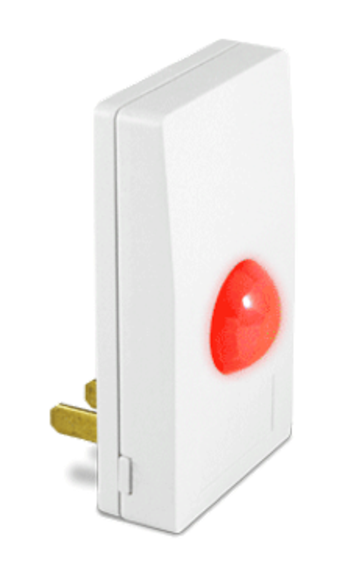
\includegraphics[keepaspectratio,angle=90]{figuras/sensor_movimento.eps}
		\caption{Modelo utilizado no projeto}
	  \end{center}

	Antes da pensar em utilizar os sensores com o sistema pronto, seriam necessários 2 sensores diferente pra medir temperatura e movimento em cada cômodo. Com este equipamento é possível ter acesso a esses dois dados apenas plugando o aparelho numa tomada $120V/60Hz$.

	O fabricante recomenda tomar alguns cuidados na instalação do sensor. Por exemplo, para se ter uma eficiência maior em detectar moimento, o sensor precisa ser instalado perpendicularmente ao eixo em que é determinado o fluxo. Conforme a figura abaixo.
	\end{figure}

	\begin{figure}[h]
	  \begin{center}
		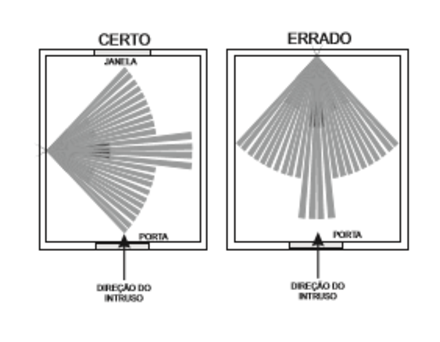
\includegraphics[keepaspectratio]{figuras/sensores_posicao.eps}
		\caption{Posição dos sensores de movimento}
	  \end{center}
	
	Isso permite que grande parte dos feixes sejam cortados e evita que algo passe despercebido. Porém, é necessário também que não haja luz solar e nem ventilação incidindo diretamente no sensor, isso pode provocar alarmes indesejados.
	
	\begin{itemize}
		\item Valor: U$\$ 69,95$.
		\item Nome: HSM200. 
		\item Quantidade: 3
	\end{itemize}
	\end{figure}

	\begin{figure}[h]
	\item Sensor de umidade no ambiente 

	  \begin{center}
		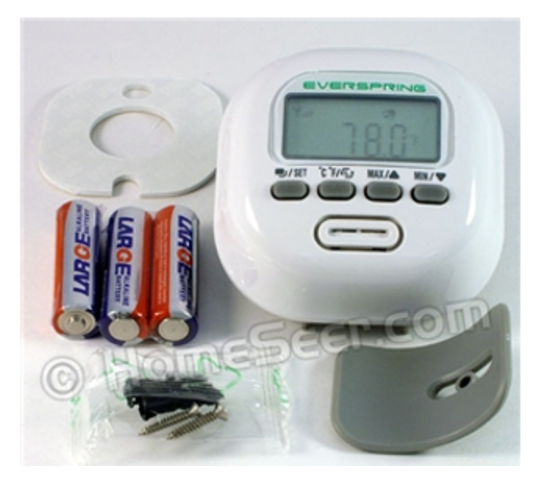
\includegraphics[keepaspectratio,scale=0.60]{figuras/sensor_umidade.eps}
		\caption{Sensor de umidade do ar utilizado no projeto}
	  \end{center}

	Este sensor é capaz de disparar funções quando atinge níveis críticos de umidade ou temperatura. Será usado em ambientes comuns para ativar umidificadores em climas secos (Umidade < 30\%). 

	\begin{itemize}
		\item Capacidade de medição de umidade: 20\% - 90\% UR.
		\item Nome: ST814-2.
		\item Preço: U$\$ 48,80$.
		\item Quantidade: 4
	\end{itemize}

	\end{figure}

	\begin{figure}[h]
	\item Ducha eletrônica
	
	Mesmo não sendo conectada à rede inteligente, a ducha inteligente é um grande adianto no que diz respeito a uso de sensores e comunicação homem-sistema.
	
	  \begin{center}
		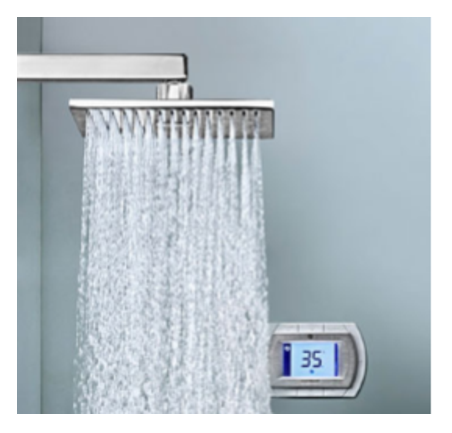
\includegraphics[keepaspectratio,scale=0.60]{figuras/ducha_inteligente.eps}
		\caption{Ducha inteligente com o painel de controle ao lado}
	  \end{center}
		
	A grande vantagem em escolher essa ducha é a capacidade que ela tem de executar as mesmas funções estabelecidas no projeto de um forma bem mais simples. Além de não ser necessário o uso de sensores, ela tem sua própria central de comando e, por ser pressurizada, reduz o consumo de água sem perder a o conforto do banho.

	\begin{itemize}
		\item Nome: Smartshower.
		\item Custo: - - - - 
		\item Quantidade: 1
	\end{itemize}
	\end{figure}
	
	\begin{figure}[h]
	\item Detector de fumaça
	
	O detector de fumaça será utilizado apensa na sala de controle, onde ficará a central do sistema. É uma medida de mater o sistema constante, a fim de evitar danos aos equipamentos em caso de incêndio ou superaquecimento.
	
	  \begin{center}
		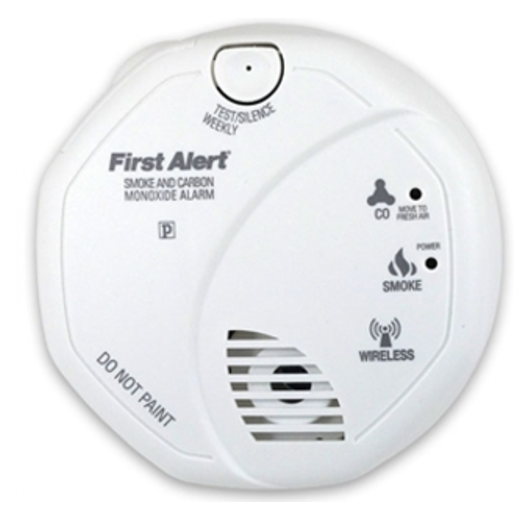
\includegraphics[keepaspectratio,scale=0.60]{figuras/detector_fumaca.eps}
		\caption{Detector de fumaça utilizado na sala de controle}
	  \end{center}

	\begin{itemize}
		\item Nome: ZCOMBO-G
		\item Custo: U$\$ 43,87$
		\item Quantidade: 1
	\end{itemize}
	
	Alguns do equipamentos passaram a não precisar mais de sensores. São eles: As cortinas, os regadores e o detector de gás de cozinha. Agora o comando de ativação dos atuadores não vem mais dos sensores, mas sim do usuário ou da máquina. 
	\end{figure}
	
	\begin{figure}[h]
	\item Smart Grid
	
	A parte do smart grid nesse Sistema conta com um medidor de consume em tempo real, e o dado é fornecido para a central. Ou seja, é possível tomar medidas de controle caso a casa esteja gastando muito.
	
	  \begin{center}
		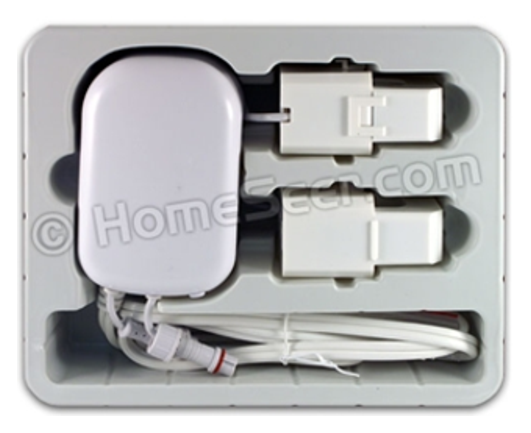
\includegraphics[keepaspectratio,scale=0.60]{figuras/medidor_instantaneo.eps}
		\caption{Medidor instantâneo do consumo total}
	  \end{center}

	\begin{itemize}
		\item Nome: DSB28-ZWUS
		\item Custo: U$\$ 94,46$
		\item Quantidade: 1
	\end{itemize}
	\end{figure}
	
	\begin{figure}[h]
	\item Câmeras
	
	Com as câmeras houve um pequeno problema: A banda de operação do Z-Wave não suporta compartilhamento de áudio e nem de vídeo. A saída mais prática é passar as informações pela internet. O próprio sistema oferece suporte à esse tipo de comunicação.
	
	  \begin{center}
		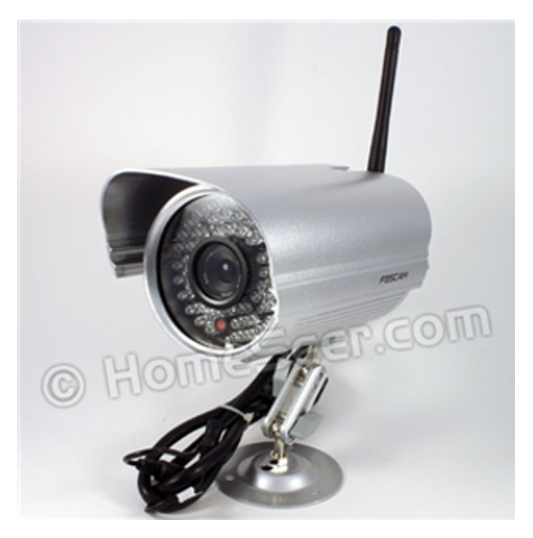
\includegraphics[keepaspectratio,scale=0.5]{figuras/camera.eps}
		\caption{Câmeras de vigilância externa}
	  \end{center}
	
	A câmera escolhida tem capacidade de filma em invravemerlho com um alcance de até 30 metros, média resolução (640x480) e ainda conta com suporte à visualização remota tanto em PC’s quanto em smartphones. O sistema oferece um programa em que a câmera só é ativada quando á movimento detectado. Ele pode ser baixado no prórpio site.

	\begin{itemize}
		\item Nome: FI8905W
		\item Custo: U$\$ 84,00$
		\item Quantidade: 8
	\end{itemize}	
	\end{figure}

\end{enumerate}

\begin{figure}[h]
	A posição dos sensores será estabelecida de acordo com a necessidade da casa e obedecendo às características exigidas pelo manual. Dessa forma, deve-se lembrar que os sensores de movimento não podem ser instalados em áreas externas, as câmeras tem ângulo de alcance de $30{^o}$ e uma distância máximo de $30m$, isso deve ser levado em conta na hora de fazer a cobertura de monitoramento da casa. Como os equipamentos tem alcance de $30m$ não será necessário o uso de repetidores, já que o lote tem justamente esse tamanho. O mapa de sensores ficou da seguinte maneira:

  \begin{center}
	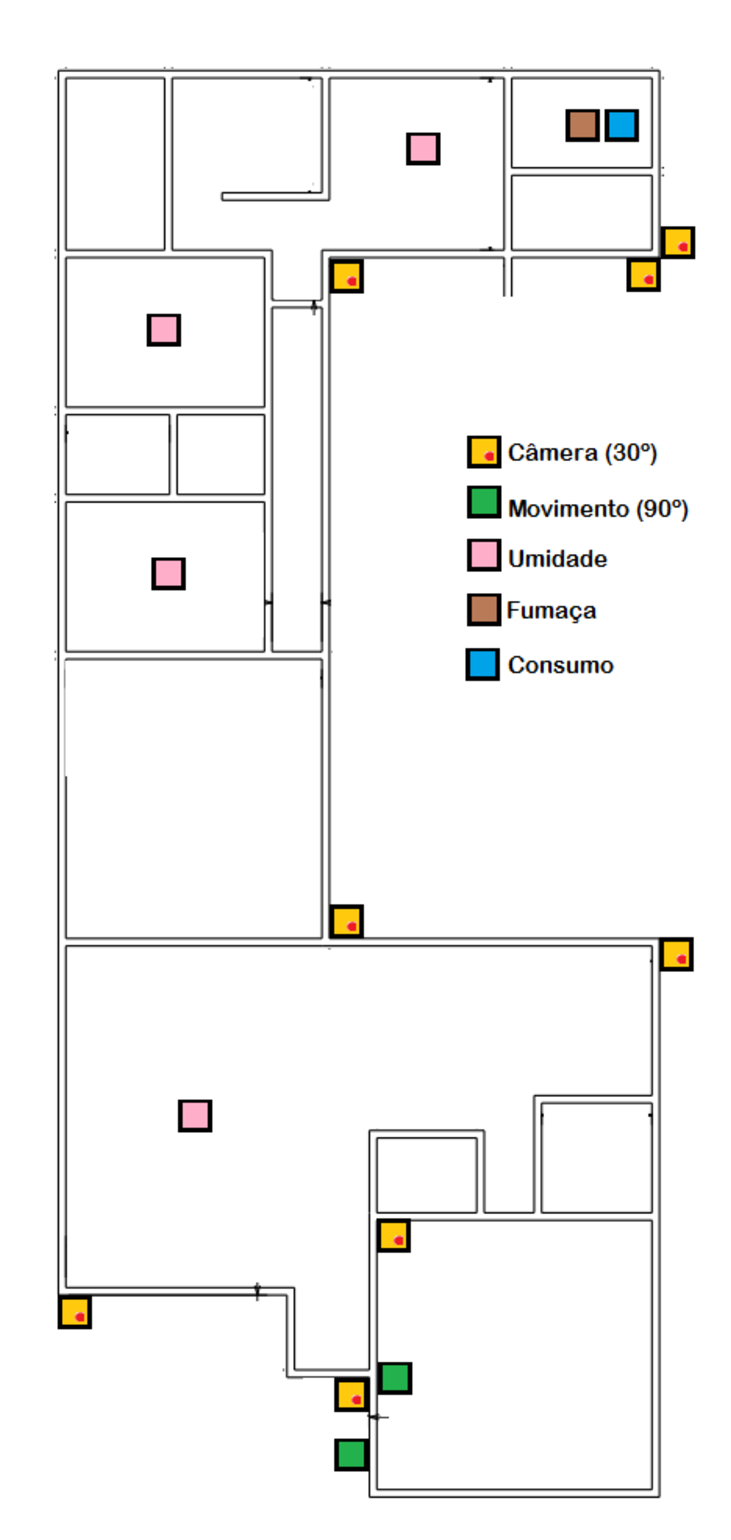
\includegraphics[keepaspectratio,scale=0.55,angle=90]{figuras/posicao.eps}
	\caption{Posição dos sensores na casa}
  \end{center}
\end{figure}


















